\topic{20}{From the lecture to the executable CPU laboratory}
\textbf{Aim.} Complete the physics-to-surrogate chain using the retained accepted CFD cases, then explain why a newly optimized shape still needs a new governing-equation calculation. Ordinary Run All performs small CPU calculations and fits; it does not launch SU2.

\begin{center}\small
\begin{tabularx}{\linewidth}{p{.16\linewidth}X X}
\toprule
Notebook stage & Algorithm and information & Inspect and interpret\\\midrule
Sections 1--4 & Pressure normalization, fixed-volume geometry and Taylor--Maccoll ODE & Units, constant volume and the analytic cone verification\\
Sections 5--9 & Geometry partition, training-only POD, ridge/GP/MLP fits & Fresh validation errors and all three methods' pressure profiles\\
Section 10 & Saved neural checkpoint, fixed normalization and stored splits & Current inference against the retained verification record\\
Sections 11--13 & Surrogate grid search and the independently solved retained design & A new proposal versus an already verified design; they are not interchangeable\\\bottomrule
\end{tabularx}
\end{center}

\textbf{What students can change.}
\begin{itemize}
\item \texttt{POD\_RANK=12}: number of pressure modes.
\item \texttt{MLP\_WIDTH=32} and \texttt{MLP\_DEPTH=2}: network capacity.
\item \texttt{MLP\_MAX\_ITER=3000}: optimization budget.
\item \texttt{MODEL\_SEED=16}: reproducible initialization.
\end{itemize}
The tanh MLP uses L-BFGS; its iteration limit is a budget, not evidence of convergence. The retained neural checkpoint is a separate fixed artifact and is not replaced by these controls.

\textbf{Algorithm.}
First preserve the 24/6/8/6 training, validation, interpolation-test and extrapolation groups. Fit the pressure mean and POD basis on the 24 training cases only, transform the geometry inputs using training statistics, and fit ridge, Gaussian-process and MLP maps to coefficients/drag. Compare candidate models on validation using the declared criterion. The new all-method plot uses the first validation case fixed in the split, so viewing it does not select an easy test case. Only then freeze the choice and inspect the existing test-waveform comparisons.

\textbf{Read a pressure comparison.}
The upper panel compares $\Cp=(p-p_\infty)/(\frac12\rho_\infty U_\infty^2)$ at the same observation line and physical axial locations. The lower panel shows signed predicted-minus-CFD $\Cp$; a phase shift of a compression peak produces opposite-sign lobes. Do not reduce the conclusion to peak error alone: shock location, expansion strength, waveform norm and pressure drag can improve differently. Every method sees the same truth and coordinate array.

\textbf{A controlled experiment.}
Compare POD ranks 6 and 12 at fixed split/seed, then widths 16 and 32 at fixed rank/depth. Record fit time, warnings, selected model, validation waveform/peak/drag errors and both positive and negative changes in the signed profiles. Choose from validation before evaluating test cases. Increasing depth and increasing the iteration ceiling simultaneously does not isolate capacity.

\textbf{The optimization boundary.}
Changing a surrogate changes the proposed optimum. The retained CFD files validate their recorded shape and conditions only: they do not validate a different proposed shape merely because the notebook can plot both. Submit the proposal's geometry coordinates and constraint values; mark it unverified until a separate accepted CFD calculation is available.

\begin{figure}[H]\centering
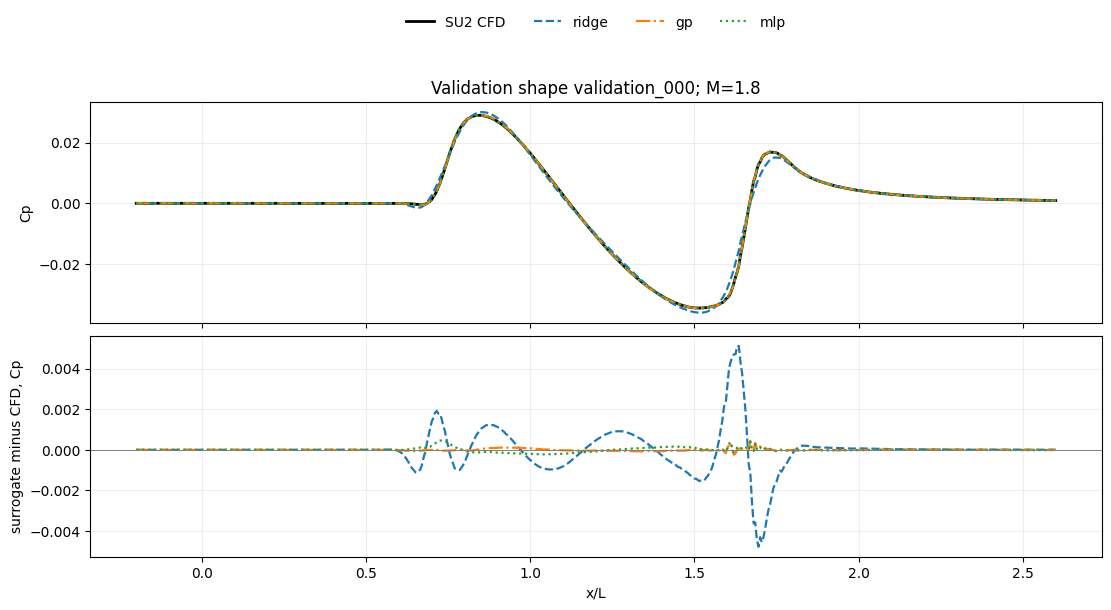
\includegraphics[width=\linewidth]{results/late_course_teaching/week16_validation_models_01.png}
\caption{First predeclared validation shape at Mach 1.8: all three fresh CPU surrogate fits share the same CFD pressure signature. Signed discrepancies expose displaced waves and amplitude errors. This plot is used for development, not as a final-test result.}
\end{figure}
